% Chapter 1
\chapter{Introduction}
\label{Chapter1}

%----------------------------------------------------------------------------------------
\newcommand{\keyword}[1]{\textbf{#1}}
\newcommand{\tabhead}[1]{\textbf{#1}}
\newcommand{\code}[1]{\texttt{#1}}
\newcommand{\file}[1]{\texttt{\bfseries#1}}
\newcommand{\option}[1]{\texttt{\itshape#1}}

%----------------------------------------------------------------------------------------
\vspace{-1cm}
\section{Background and motivation} \label{sec:background_motivation}


The extensive use of PFAS in various industries and consumer products has led to their widespread presence in the environment. PFAS have been detected in various environmental media, including water, soil, and air, as well as in the tissues of wildlife and humans. Due to their chemical stability and resistance to natural degradation processes, PFAS can persist in the environment for decades, posing long-term exposure risks. Their persistence, combined with their ability to bioaccumulate in living organisms, raises serious concerns regarding human health and environmental sustainability~\cite{PFAS_in_animals_humans, PFAS_livestock, PFAS_environ_impacts_health, PFAS_in_water, PFAS_in_drinking_water}.

There is growing evidence that exposure to PFAS substances is associated with a range of adverse health effects. Epidemiological studies have linked PFAS exposure to an increased risk of certain cancers, liver damage, immune systems suppression, thyroid dysfunction, and developmental issues in children~\cite{PFAS_cancers_1, PFAS_cancers_2, PFAS_fatty_liver_USA, PFAS_immune_suppression, PFAS_developmental_issues}.These health concerns are particularly alarming given the widespread presence of PFAS. Studies indicating that nearly all individuals in industrialized nations have detectable levels of these substances in their blood~\cite{PFAS_Italy}. The potential for chronic health effects, combined with the persistence and bioaccumulative nature of PFAS, has heightened intensified public and scientific interest in understanding and mitigating

The regulatory landscape for PFAS is evolving rapidly as governments and environmental agencies respond to the growing body of evidence regarding their environmental and health impacts. In the United States, for example, the Environmental Protection Agency (EPA) has begun establishing health advisories and regulatory limits for certain PFAS compounds in drinking water. Similar efforts are underway in other countries, particularly within the European Union, where restrictions on specific PFAS compounds are being implemented. However, the vast number of PFAS substances, combined with limited toxicological data for many of them, presents significant challenges for regulatory authorities. 

%----------------------------------------------------------------------------------------
\section{Per- and polyfluoroalkyl substances} \label{sec:pfas_intro}

PFAS substances are a group of organic compounds characterized by carbon chains bonded to fluorine atoms. Figure \ref{structure_chapter_2} provides the names, abbreviations, and 2D structures of the more commonly studied PFAS. According to the Organization for Economic Co-operation and Development (OECD)’s latest definition, PFAS are fluorinated substances that contain at least one fully fluorinated methyl or methylene carbon atom ~\cite{2}. PFAS can be classified as short-chain (≤ seven carbon atoms) or long-chain (≥ eight carbon atoms) compounds. Long-chain PFAS are often referred to as “legacy” compounds due to their extensive history of study. The most thoroughly researched long-chain PFAS are perfluorooctane sulfonate (PFOS) and perfluorooctanoic acid (PFOA). Production of these compounds was discontinued in several countries (e.g., the United States in the 2000s) due to their adverse health effects~\cite{2,3}.

The chemical structure of PFAS, particularly its carbon–fluorine (C–F) bonds, includes some of the strongest bonds in organic chemistry. This exceptional bond strength contributes to PFAS’s high resistance to chemical, thermal, and biological degradation. This allows PFAS to persist in the environment and in the human body, where they are difficult to eliminate. PFAS are non-flammable, non-corrosive, and resistant to combustion, degradation, and most chemical reactions. Furthermore, PFAS molecules typically possess both hydrophobic and hydrophilic ends, giving them unique surfactant properties. Their long biological half-lives result in bioaccumulation over time, further complicating efforts to mitigate their impact on human health and the environment. While the production of certain PFAS, such as PFOA and PFOS, was halted in countries like the United States due to their toxicity concerns, these substances still pose significant environmental and health risks~\cite{PFOA_PFOS_risk}.

\begin{figure}[H]
\centering
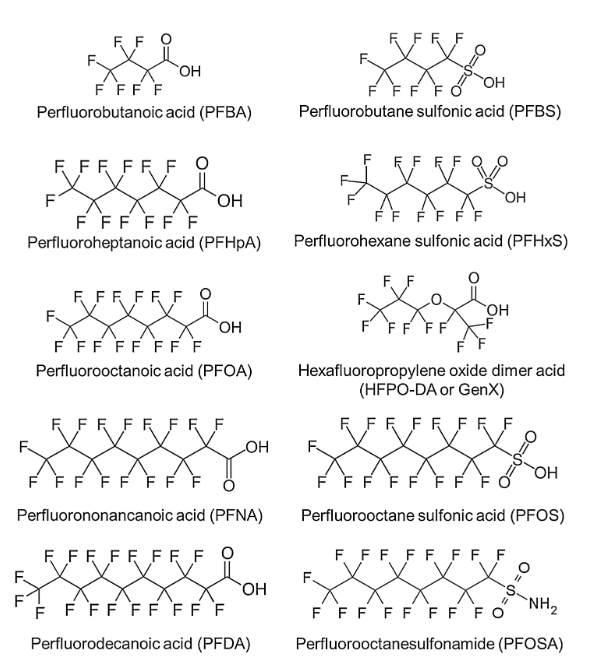
\includegraphics[width=\textwidth,height=\textheight,keepaspectratio]{Figures/structure_chapter_2.png}
\caption{Two-dimensional (2D) chemical structures of selected PFAS and related compounds \cite{structures_graphic}}
\label{structure_chapter_2}
\FloatBarrier
\end{figure}

%----------------------------------------------------------------------------------------
\clearpage
\subsection{Uses and potential risks} \label{sec:uses_risks}

PFAS substances are a group of synthetic compounds widely used in industrial processes due to their resistance to degradation, surfactant properties, and thermal and flame resistance. Their water- and grease-repellent properties make them ideal for food packaging, non-stick cookware, and waterproof textiles. Beyond these applications, PFAS are also found in paints, adhesives, electrical wire insulation, detergents, fire-resistant materials, carpets, and even cosmetics~\cite{3,4}.

One of the most concerning effects of PFAS compounds exposure is their potential impact on thyroid health. Thyroid hormones play a key role in regulating metabolism, and proper thyroid function is associated with cardiovascular health, fertility, and fetal neurodevelopment. Studies have suggested that PFAS may disrupt thyroid hormone regulation, which could potentially affect pregnancy outcomes and the development of fetuses and young children ~\cite{3}.

%----------------------------------------------------------------------------------------
\subsection{Environmental and health concerns} \label{sec:env_health_concerns}

The widespread use of PFAS in various industries, coupled with the chemicals’ stability, has led to significant environmental contamination. PFAS compounds have been detected in surface water, groundwater, soil, and air. Their solubility in water and resistance to degradation allow them to travel long distances from their original source(s), contributing to their global distribution in the environment~\cite{Sweden_distribution}.

Recent epidemiological studies have linked exposure to certain PFAS compounds with adverse health effects. These risks are further compounded by PFAS’s ability to accumulate in the human body over time, particularly in the blood, liver, and kidneys, due to their long biological half-lives. Consequently, even low-level, long-term exposure to PFAS can lead to serious health consequences. Many legacy PFAS, such as PFOA and PFOS, have accumu- lated in the environment, as well as in animals and humans. Mixtures of legacy and newer PFAS continue to be detected in the environment, including in global food and water supplies. The biological half-lives of legacy PFAS in human serum are approximately four years for PFOA, five years for PFOS, and eight and a half years for PFHxS. The biological half-lives of newer PFAS compounds are less well understood, though available studies suggest that they are excreted at significantly faster rates~\cite{4}.

Full defluorination (DeF) or mineralization of PFAS is necessary to eliminate fluoride contamination completely. However, current technologies can only partially defluorinate a limited range of PFAS compounds. In 2023, the U.S. EPA established new drinking water standards for perfluorooctanesulfonic acid (PFOS) and perfluorooctanoic acid (PFOA) at 4.0 parts per trillion (ppt). Achieving this near-zero threshold will require technological innovations that enable the complete defluorination of parent PFAS compounds, rather than merely degrading them. DeF specifically refers to the percentage of fluoride ions released from PFAS molecules. Full DeF is critical because partial defluorination can lead to the formation of  potentially more toxic and persistent short-chain byproducts that are more likely to bioaccumulate in animals and humans~\cite{6}.

%----------------------------------------------------------------------------------------
\subsection{Regulatory challenges and research directions} \label{sec:reg_challenges}

Because of the persistence and toxicity of PFAS, regulatory agencies worldwide have started to implement guidelines and regulations that limit human and environmental exposure. For example, the U.S. EPA has issued health advisories for PFOA and PFOS in drinking water. Although these advisories are not legally enforceable, they are currently under review for potential revision. Similarly, several European Union countries have restricted the use of certain PFAS in consumer products and industrial applications. Despite these efforts, the vast number of PFAS compounds, combined with the lack of comprehensive toxicological data for many of them, continue to pose significant challenges for regulatorss~\cite{PFAS_regulators, PFAS_regulators_2, PFAS_regulators_3}.

Ongoing research is focused on developing more effective methods for detecting and quantifying PFAS in environmental samples and exploring potential remediation strategies. Analytical techniques such as liquid chromatography–mass spectrometry (LC–MS/MS) have become the gold standard for PFAS detection due to their high sensitivity and specificity~\cite{PFAS_detection_1, PFAS_detection_2, PFAS_detection_3, PFAS_detection_4}. Nevertheless, detecting PFAS at environmentally relevant concentrations remains challenging, particularly for emerging PFAS compounds that are not well characterized. 

In terms of remediation, conventional water treatment technologies, such as activated carbon filtration and ion exchange, have been somewhat effective at removing PFAS from contaminated water sources. However, these methods often lack the capacity to address the full spectrum of PFAS compounds present in the environment. Consequently, advanced treatment methods, including high-pressure membrane filtration, advanced oxidation processes, and electrochemical degradation, are being investigated as potential solutions to this complex issue~\cite{PFAS_membrane_filtration, PFAS_oxidation_1, PFAS_oxidation_2}.

% ----------------------------------------
% ----------------------------------------
% ----------------------------------------
\clearpage
\subsection{Methods for determining biological and physicochemical \\properties}

Chemical safety evaluations rely on an understanding of key properties, such as half-life, protein binding, solubility, and membrane permeability. These parameters have traditionally been assessed through \textit{in vivo} studies (i.e., animal testing) or \textit{in vitro} assays (e.g., cell cultures).). In recent years, in silico techniques, particularly qualitative and quantitative structure–activity/property relationships, have gained importance. These techniques offer faster, more ethical and more cost-effective alternatives to laboratory testing. They also enable preliminary hazard screening in scenarios with limited data \cite{Gkika2023, Cherkasov2014}.

\subsection{QSAR/QSPR models for PFAS}

Recent technological advancements, particularly in computing, have led to a steady increase in the use of computer-based approaches, commonly referred to as \textit{in silico} methods, in chemical hazard assessment. Two major categories of \textit{in silico} approaches can be distinguished: (1) qualitative structure-activity/property relationship methods (SAR/SPR also known as [Q]SAR/[Q]SPR) and (2) quantitative structure-activity/property relationship methods (QSAR/QSPR). Both types of methods aim to establish a link between the structural features of a group of chemical compounds and their biological activity (e.g., acute toxicity to \textit{Daphnia magna}) or physicochemical property (e.g., water solubility), through the development of appropriate mathematical models. The primary difference between these two approaches is the type of output they generate. [Q]SAR/[Q]SPR models produce categorical (i.e., discrete) outcomes, whereas QSAR/QSPR models yield numerical (i.e., continuous) predictions. Qualitative methods are generally preferred in the early stages of analysis because they enable the rapid classification of chemical compounds into distinct classes. For example, they can distinguish between biologically active and inactive compounds. This classification typically involves assigning labels such as “toxic” or “non-toxic.”\cite{NevesB}\cite{TsuiM}

The [Q]SAR/[Q]SPR methodology, schematically presented in Figure \ref{fig:SAR_modeling_flowchart}, consists of six main stages, which are briefly described below. 

\begin{figure}[H]
    \centering
    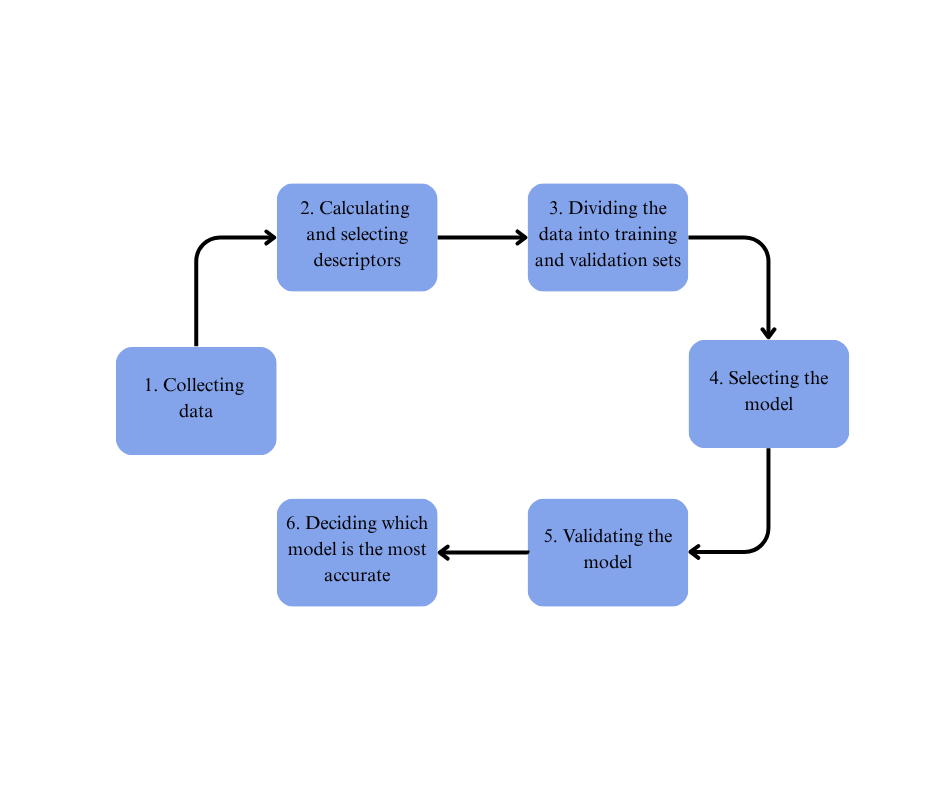
\includegraphics[width=\textwidth,height=\textheight,keepaspectratio]{Figures/SAR.png}
    \caption{[Q]SAR modeling flowchart (own work)}
    \label{fig:SAR_modeling_flowchart}
\end{figure}

The first step in the [Q]SAR/[Q]SPR modeling process is collecting data from experiments, literature, or relevant databases. Next, molecular descriptors are calculated. These descriptors play an important role in [Q]SAR/[Q]SPR modeling because they provide a mathematical representation of the various structural and physicochemical properties of molecules. Depending on how they are obtained, descriptors fall into two categories: (1) experimental, which are determined through laboratory measurements (e.g., water solubility), and (2) theoretical, which are calculated based on chemical composition, structural topology (i.e., the arrangement of atoms in a molecule), or derived from quantum-mechanical calculations based on the 3D molecular structure (e.g., polarizability). A well-chosen descriptor exhibits continuous variability and, most importantly, captures subtle changes in molecular structure \cite{MauriA}. The set of descriptors selected for developing a [Q]SAR/[Q]SPR model should facilitate mechanistic interpretation by linking structural variations to observed changes in biological activity. In other words, the descriptors should provide insight into the underlying mechanism of action, such as the toxic effect of a chemical compound within a biological system.


The third step in the [Q]SAR/[Q]SPR modeling process is to split the collected dataset into two subsets:

\begin{enumerate}
    \item \textbf{The training set}, which is used to build the model. This involves defining logical rules or decision boundaries to classify objects (i.e., compounds) into categories (i.e., two or more classes), in the case of qualitative models;
    \item \textbf{The test set} (also known as validation set), which is used to evaluate the model’s predictive accuracy for compounds not included in the training phase.
\end{enumerate}

The fourth step is selecting an appropriate machine learning (ML) algorithm. This is a crucial step because the modeling technique must align with the nature and complexity of the dataset to capture meaningful relationships. Using an inappropriate ML method can significantly reduce predictive accuracy and increase misclassification rates. Another challenge is the wide array of available modeling techniques, each of which requires tuning specific parameters.

Before a developed [Q]SAR/[Q]SPR model can be applied in practice, it must undergo rigorous validation. This step is essential for assessing the model’s reliability in predicting biological responses or physicochemical properties, for compounds not involved in model development. \cite{NevesB}\cite{Jaganathan}\cite{Polishchuk}

Relatively few [Q]SAR/[Q]SPR models focus specifically on PFAS, primarily due to the limited availability of high-quality experimental data. Existing models often rely on simple one- or two-dimensional (1D or 2D) descriptors, such as molecular weight or n-octanol-water partition coefficient (logP), and tend to overlook more detailed electronic structure descriptors, such as the energy difference between the highest occupied molecular orbital (HOMO) and lowest-unoccupied molecular orbital (LUMO) (HOMO–LUMO gap) or chemical potential \cite{BlakeFenton2020, Gkika2023}. This underscores the necessity of incorporating more sophisticated descriptors to more accurately capture the factors influencing PFAS persistence and toxicokinetics. However, it should be noted that quantum-chemical modeling of PFAS poses challenges, especially when selecting the optimal combination of functionals, basis sets, and polarization and/or diffuse functions. The wide variety of these parameters makes determining the most suitable setup for accurately modeling this unique class of compounds difficult.

 
Therefore, selecting the most appropriate levels of theory adds complexity to geometry optimization, descriptor calculation, and, ultimately, [Q]SAR/[Q]SPR model development. Options include various functionals (e.g., \texttt{B3LYP}, \texttt{M06‑2X}, \texttt{$\omega$B97X-D)}, basis sets (e.g., \texttt{6‑31G}, \texttt{6‑31++G}, \texttt{cc-pVTZ}), and descriptor types (e.g., electronic, geometric, and thermodynamic). Each combination involves trade-offs between computational cost and the accuracy of the resulting descriptors. An optimal workflow should balance model performance and computational feasibility, especially for large-scale screening applications \cite{Gkika2023, Cherkasov2014}.

% ----------------------------------------
% ----------------------------------------
% ----------------------------------------
\chapter{Research hypothesis and objectives}

Given the limitations of existing in silico models, which often rely on simple 1D or 2D descriptors and fail to capture electronic structure, this section outlines the key research questions and hypotheses that guide this master’s thesis.

This thesis primary aims to investigate whether descriptors derived from DFT can improve the prediction of PFAS half-life categories when combined with molecular descriptors generated using RDKit \cite{rdkit} and Open Babel \cite{openbabel}. To explore this, we pose the following three specific research questions:

\begin{enumerate}
  \item Does combining DFT-derived descriptors (i.e., electronic, geometric, and thermodynamic) with RDKit/Open Babel descriptors improve the accuracy with which PFAS are classified into half-life categories compared to models that do not incorporate descriptors based on optimized 3D structure?
  
  \item How does the choice of DFT functional (\texttt{B3LYP}, \texttt{M06‑2X}, \texttt{\(\omega\)B97X‑D}) and basis set (\texttt{6-31G(d,p)}, \texttt{6-31++G(d,p)}, \texttt{cc-pVTZ}) ) influence the robustness of the descriptors and the overall performance of the model, while considering computational time?
  
  \item Is it possible to identify an optimal combination of ML method and descriptor set that balances predictive accuracy with computational efficiency?
\end{enumerate}

Based on these questions, we formulated the following research hypotheses:

\begin{itemize}
  \item H1: Classification models incorporating DFT-derived descriptors will outperform —or at least match—the predictive accuracy of models using only 1D and 2D descriptors, potentially with lower model complexity.
  
  \item H2: The quality of the [Q]SPR models varies depending on the chosen DFT method, however, more computationally expensive methods do not necessarily yield better predictive performance.
  
  \item H3: A combination of DFT method and descriptor set exists that offers high classification performance at a significantly reduced computational cost compared to high-level DFT calculations.
  
  \item H4: The choice of ML algorithm (e.g., k-NN, DT, XGB) significantly impacts both classification performance and model interpretability.
\end{itemize}

To test these hypotheses, the following objectives have been defined:

\begin{enumerate}
  \item Perform DFT optimizations of PFAS structures using the selected functionals and basis sets, and record the computational time required for each.
  
  \item Generate electronic, geometric and thermodynamic descriptors from the optimized molecular geometries.
  
  \item Integrate the DFT-derived descriptors with the original data derived from \cite{dataset_source} , including PFAS half-lives and biological descriptors.
  
  \item Perform feature selection and develop classification models to classify PFAS based on toxicokinetic half-life.
  
  \item Evaluate model performances across different combinations of DFT-derived descriptor sets and ML algorithms to identify the optimal trade-off between accuracy and computational cost.
\end{enumerate}

Through this research workflow, we aim to improve our understanding of how molecular structure, particularly electronic properties, affects PFAS environmental persistence. Additionally, the master’s thesis seeks to deliver a scalable, practical computational workflow for predicting the environmental and human health risk of legacy and emerging PFAS compounds.

